\chapter{Qualification of the Electronics}
\label{chap:II-4-qualification}

  To prepare the DAQ system for the slice test, the electronic components need to be tested and qualified. For the VFAT2s, qualification procedures have to be developed to characterize the analog front-end of each chip, record their response to calibration pulses, and optimize the parameters to achieve uniformity over the entire detector. For the GEB, qualification means ensuring that no shorts are present and that the integrity of the signals is kept over the full length of the board. Finally, the system as a whole needs to be tested against communication errors or readout problems. \\

  In this chapter, we present the algorithms we have developed to test and qualify the various systems which rely on the firmware and software development made for the test beam. We detail the calibration procedure of the analog front-end of the VFAT2 which has never been done before. Next, we describe the GEB testing PCB which we have created in order to test the communication through the GEB. Finally, we talk about the script used to test the system as a whole which is employed at CERN and in various research laboratories to set up DAQ systems for future developments.

  \section{Qualification of the VFAT2s}

    The qualification process of the VFAT2s has been automated using Python scripts relying on IPBus to run the various procedures using the dedicated firmware modules of the OptoHybrid. The aim of this tools is to reject faulty chips and record the parameters of the analog front-end which slightly vary from component to component.

    \subsection{Identification of Faulty Channels}

      The first step of the procedure is to run a threshold scan for each channel to reveal those that are not responding or that are noisy. To do so, the tools use the threshold scan module of the firmware that relies on tracking data to access the full granularity information. Figure \ref{fig:II-4-threshold} is a two-dimensional graph plotting the evolution of the noise level for each channel as a function of the VFAT2 threshold in VFAT2 units. As can be seen, one of the channels appears to be damaged as it does not display any change during the whole scan and remains empty. From this result, the VFAT2 would be disqualified and not used for data taking. If performing these scans on instrumented VFAT2s, the results can be used to mask faulty channels and regain acceptable operational conditions.

      \begin{figure}[h!]
        \centering
        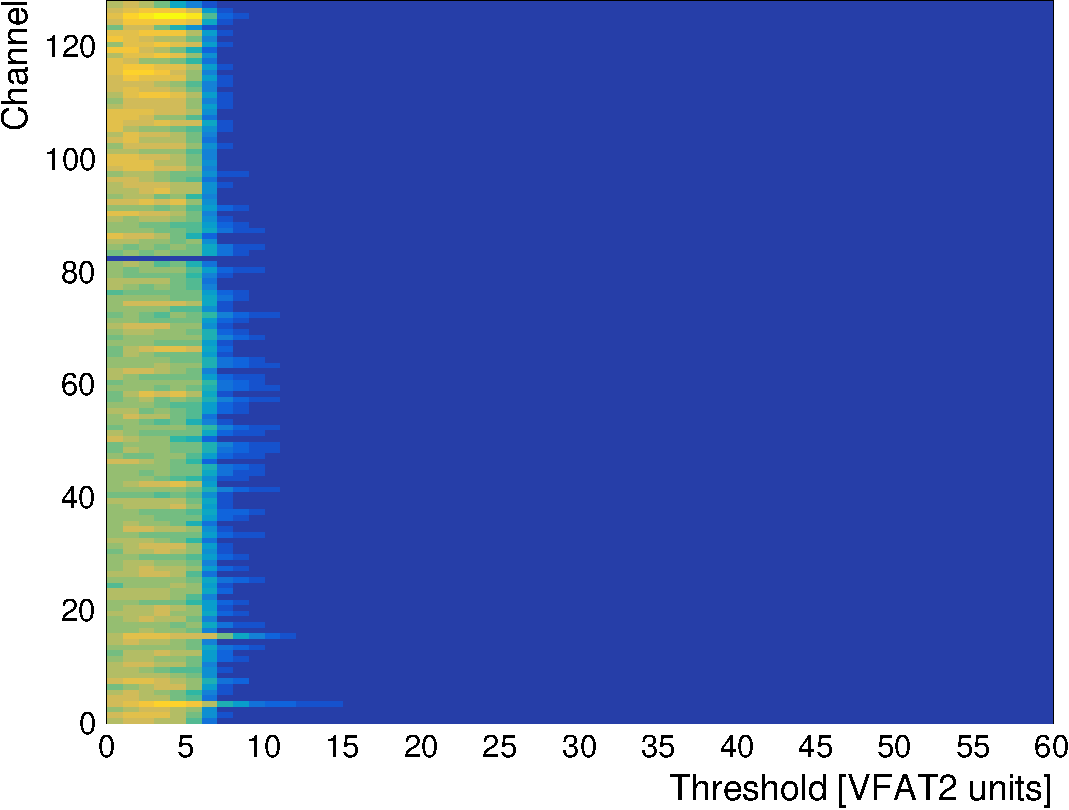
\includegraphics[width=0.5\textwidth]{img/plots/cThreshold_Channel-crop}
        \caption{Two-dimensional graph plotting the evolution of the noise level for each channel as a function of the VFAT2 threshold in VFAT2 units.}
        \label{fig:II-4-threshold}
      \end{figure}

    \subsection{Front-end Currents and Voltages}

      Following the threshold scan, the procedure reads out the currents and voltages that are produced by the VFAT2 to bias its analog front-end. When writing values in the 8-bit registers defining the threshold and other parameters, a conversion to an analog value is performed inside the chip which will vary from component to component. It is therefore essential to record the results of each chip. In order to access the analog signals inside the VFAT2, two analog signals are sent out: one for the voltage reference and one for the current reference. These lines are routed on the GEB and transmitted to the OptoHybrid which uses an ADC to digitize the information. To fit the window of operation of the ADC, which has a range of 0 V to 1 V, the voltage signal is sent through a voltage divider and the current signal is measured over a resistor. Figure \ref{fig:II-4-adc} plots the ADC counts, current values on the left, and voltage values on the right of each settable register of the VFAT2 as a function of the 8-bit value written in the register. \\

      \begin{figure}[h!]
        \centering
        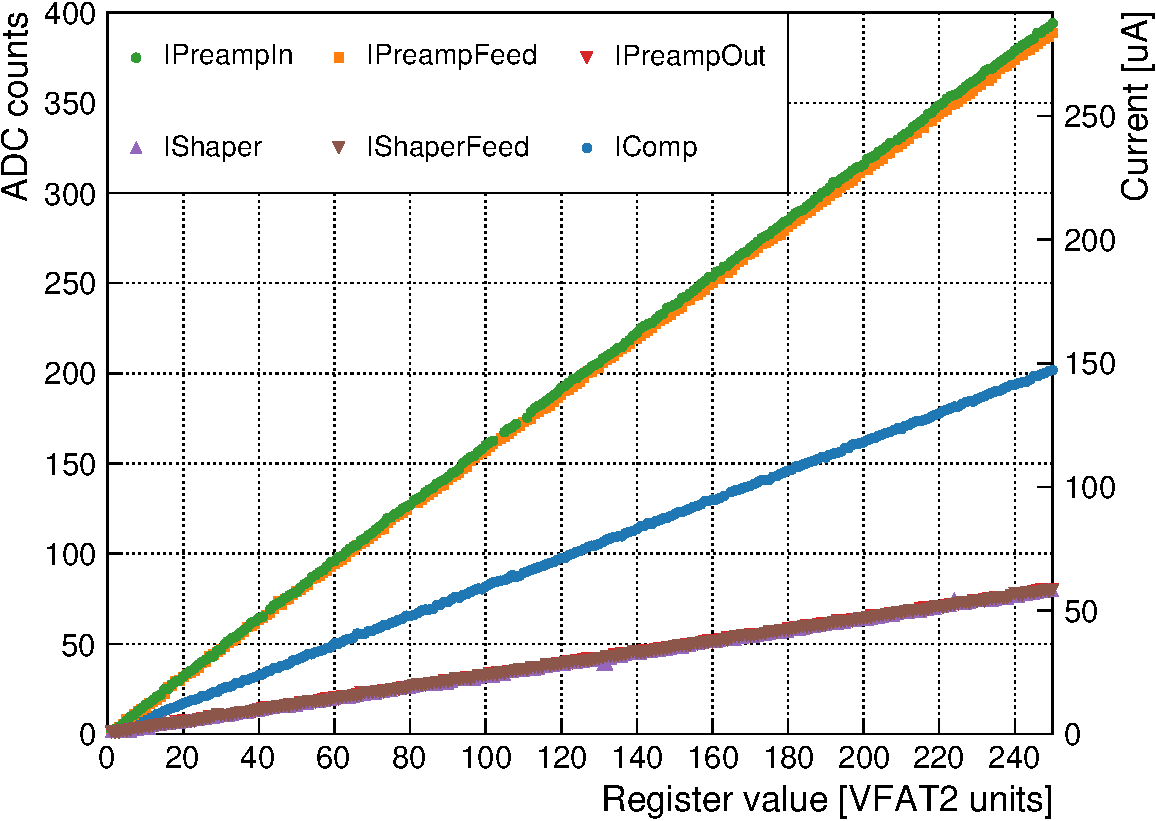
\includegraphics[width=0.49\textwidth]{img/plots/cADC_Current-crop}
        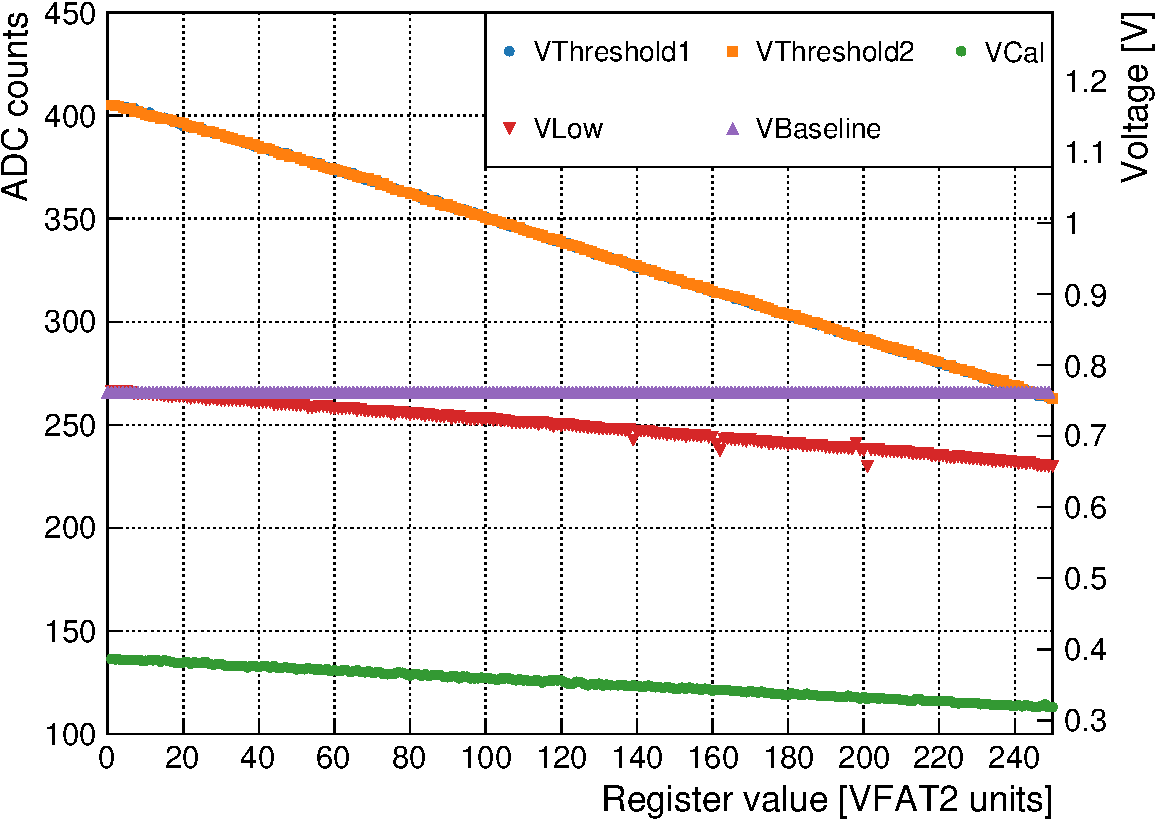
\includegraphics[width=0.49\textwidth]{img/plots/cADC_Voltage-crop}
        \caption{Plots of the ADC counts, current values on the left, and voltage values on the right of each settable register of the VFAT2 as a function of the 8-bit value written in the register.}
        \label{fig:II-4-adc}
      \end{figure}

      All but one of the current based registers are related to the amplification and shaping of the analog signal. They power the front-end and are used to define the length of the tail of the signal shape, the rise time of the distribution, etc. The remaining register, IComp, defines the amount of current delivered to the comparator which in turn influences the response time of the latter. These parameters are set to default values provided by the reference manual of the VFAT2. \\

      The voltage based registers are used for the comparator and the calibration modules. The VThreshold1 and VThreshold2 signals are those defining the threshold on the strips. By design, VFAT2 can handle positive and negative pulse and provides one threshold register for each polarity. During operations, one of the registers is set to zero and the other one is used to adjust the threshold, meaning that a single parameter is used. The VBaseline, VCal, and VLow registers are used to define the amplitude of the calibration pulse sent to the channels. Figure \ref{fig:II-4-injection} shows a diagram of the injection and calibration circuit of the VFAT2. The amplitude of the calibration pulse is equal to the difference between VBaseline which has a fixed value and VLow which is programmable. The output pulse is sent to one channel over a capacitor of 100 fF resulting in a pulse amplitude in term of charge of
      \begin{equation}
        \label{eq:II-4-injection}
        Q = 100 \ \text{fF} \times \left(\text{VBaseline} - \text{VLow} \right) .
      \end{equation}

      \begin{figure}[h!]
        \centering
        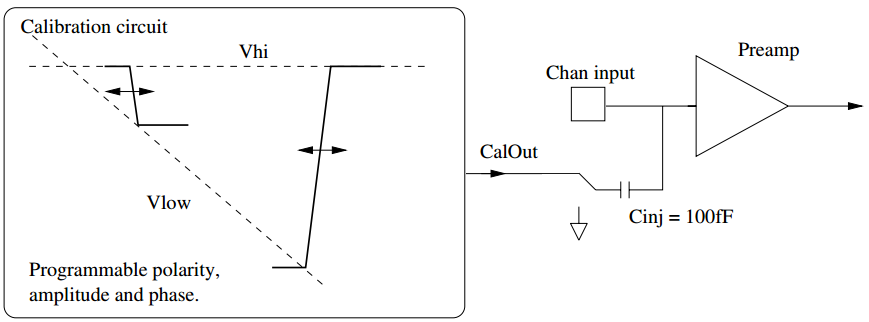
\includegraphics[width=0.8\textwidth]{img/II-4-qualification/injection.png}
        \caption{Diagram of the injection and calibration circuit of the VFAT2 highlighting the path of the calibration pulse towards a given channel \cite{Aspell:1267947}.}
        \label{fig:II-4-injection}
      \end{figure}

      By inserting the values of VBaseline and VLow in Equation \ref{eq:II-4-injection}, a range of injected charge can be computed and qualitatively compared to the one given in the VFAT2 specifications \cite{Aspell:1267947}. The latter states a range of -2 fC to 18.5 fC with a slope of 0.08 fC while the former results in a range of -0.9 fC to 20 fC with a slope of 0.08 fC. The agreement between both results helps to validate the methodology used during the calibration routines.

    \subsection{Front-end Calibration}

      Using the results from the ADC, the script can determine what amount of charge is injected during the calibration phase of the VFAT2 upon reception of a CalPulse fast command. With this, it is possible to produce s-curves which for a given threshold indicate at which amplitude of the calibration pulse a signal becomes visible. Figure \ref{fig:II-4-scurve} plots the hit-to-event ratio as a function of the calibration pulse height in VFAT2 units for a threshold of 25. The calibration pulse height refers to the value written in the VLow register which linearly affects the charge deposited on the channels. The graph shows that below a value of 40 no signal is detected due to the threshold level. The turn-on of the curve is defined as the value for which 50\% of hit-to-event ratio is reached and is in this case equal to 44. \\

      \begin{figure}[h!]
        \centering
        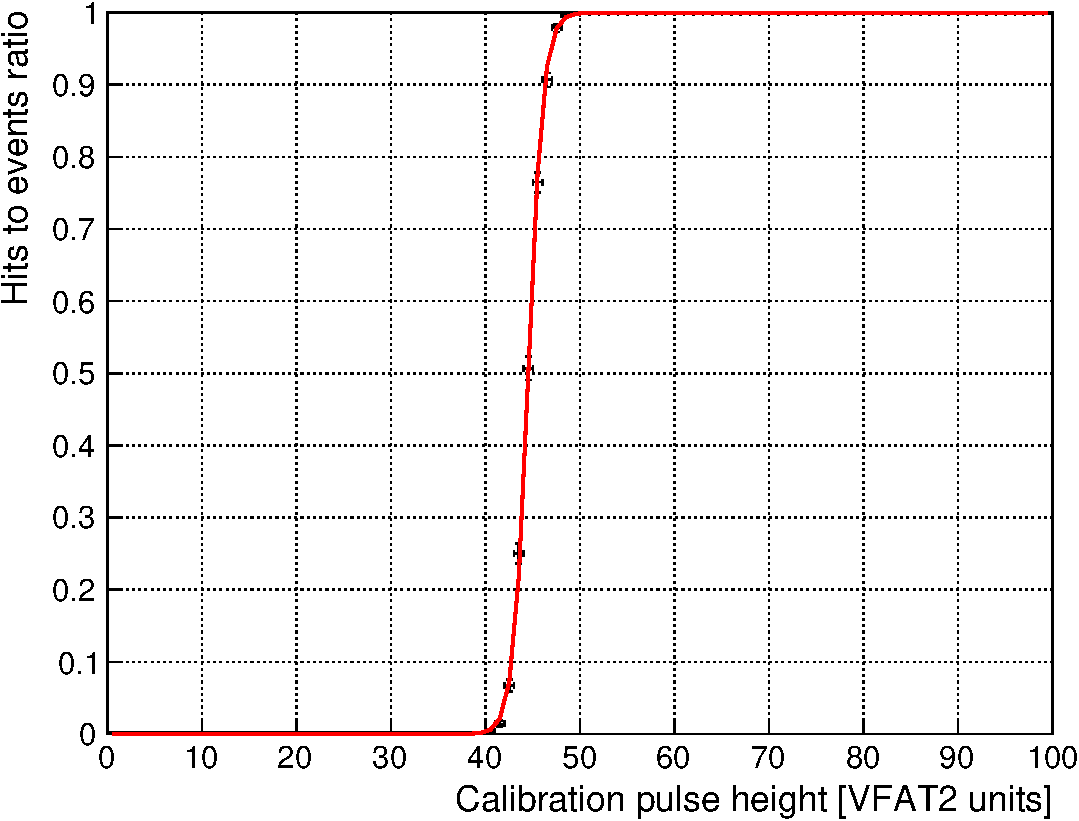
\includegraphics[width=0.5\textwidth]{img/plots/cSCurve_T25-crop}
        \caption{Plot of the hit-to-event ratio as a function of the calibration pulse height in VFAT2 units for a threshold of 25.}
        \label{fig:II-4-scurve}
      \end{figure}

      The operation is then repeated for various threshold values and the turn-on value is extracted automatically using a logistic function to fit the curve. The equation of the function is as follows
      \begin{equation}
        \label{eq:II-4-logistic}
        f(x) = \frac{1}{1 + e^{-k \left( x - x_0 \right)}}
      \end{equation}
      where $ x_0 $ is the value of the midpoint or turn-on, and $ k $ is the steepness of the slope. Figure \ref{fig:II-4-scurves} is a collection of s-curve scans for various thresholds on the left which can be translated to a plot of the calibration pulse height of the turn-on in VFAT2 units and current as a function of the threshold in VFAT2 units on the right. \\

      \begin{figure}[h!]
        \centering
        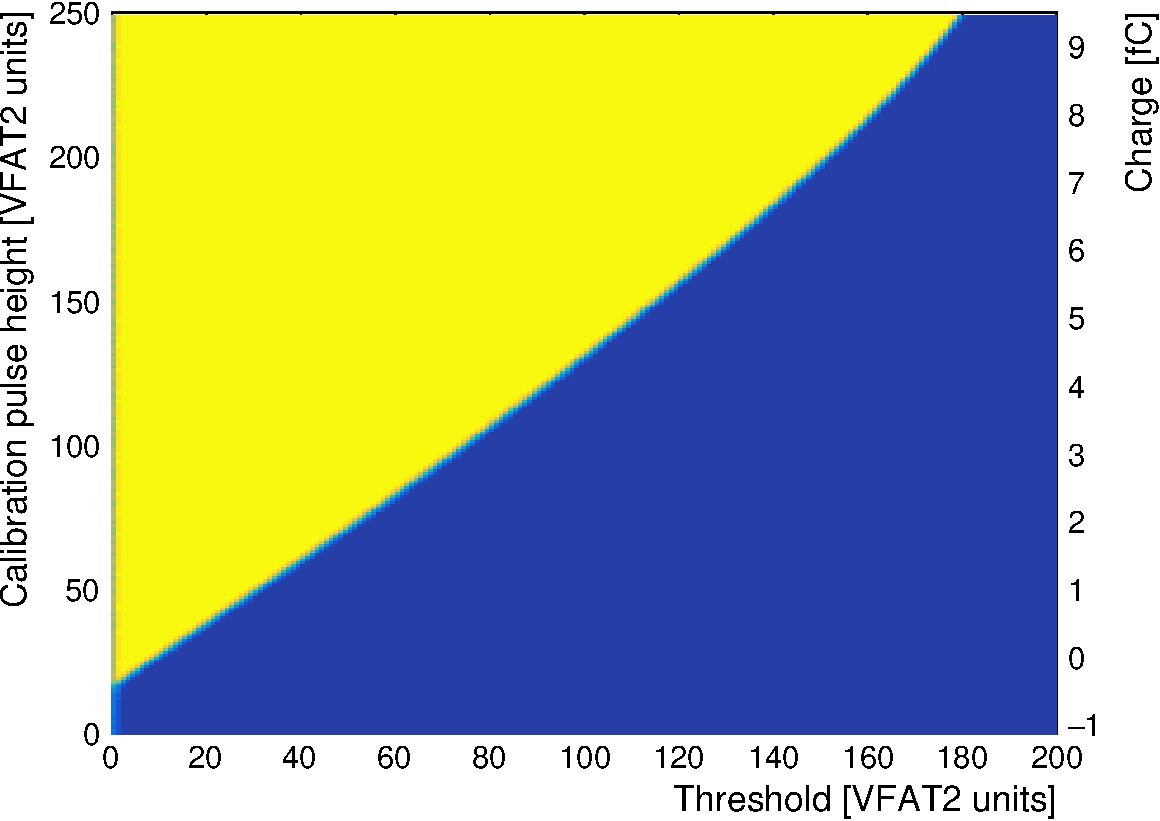
\includegraphics[width=0.49\textwidth]{img/plots/cSCurve_ThresholdVCal-crop}
        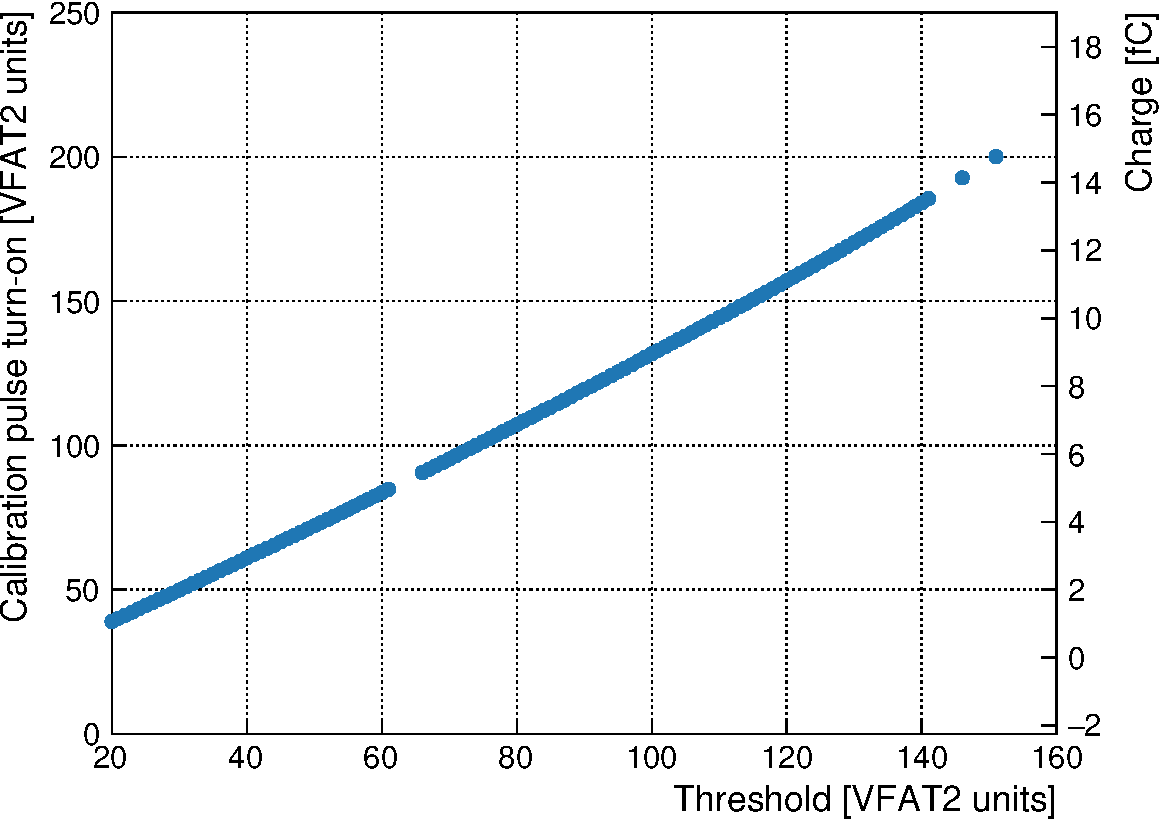
\includegraphics[width=0.49\textwidth]{img/plots/cSCurve_TurnOn-crop}
        \caption{Left: collection of s-curve scans for various thresholds with corresponding curent values. Right: plot of the calibration pulse height of the turn-on in VFAT2 units and current as a function of the threshold in VFAT2 units.}
        \label{fig:II-4-scurves}
      \end{figure}

      Using these results, the threshold value applied on the strips can be converted to a charge, which is of importance to compute the equivalent noise charge of the system. This is the amplitude of the noise in terms of electrons, which can easily be compared to the signal induced by the particles which is often expressed in femtocoulombs. The results presented here above are in agreement with those obtained during the initial qualification of the VFAT2 \cite{Aspell:1267947} both displaying a qualitative charge range of -2 fC to 18 fC.

    \subsection{Front-end equalization}

      The results obtained in the previous procedures were values averaged on all the strips. However, channels display a dispersion around the central value which induces a bias as the effective threshold is not constant across the chip. To eliminate this effect, it is possible to equalize the response of the front-end by using channel by channel programmable registers. Each of them is equipped with a programmable register which slightly adjusts the threshold value. The equalization procedure used to align the front-ends starts by applying a given value to the common threshold register and sets all channel registers to zero. It then performs s-curve scans for each channel. The operation is repeated but with the channel registers set to their maximum value. Figure \ref{fig:II-4-trim} plots the s-curve scans for each channel with the minimum value of the channel registers on the left and the maximum value on the right. The two plots obtained this way are very similar with only the turn-on value changing. \\

      \begin{figure}[h!]
        \centering
        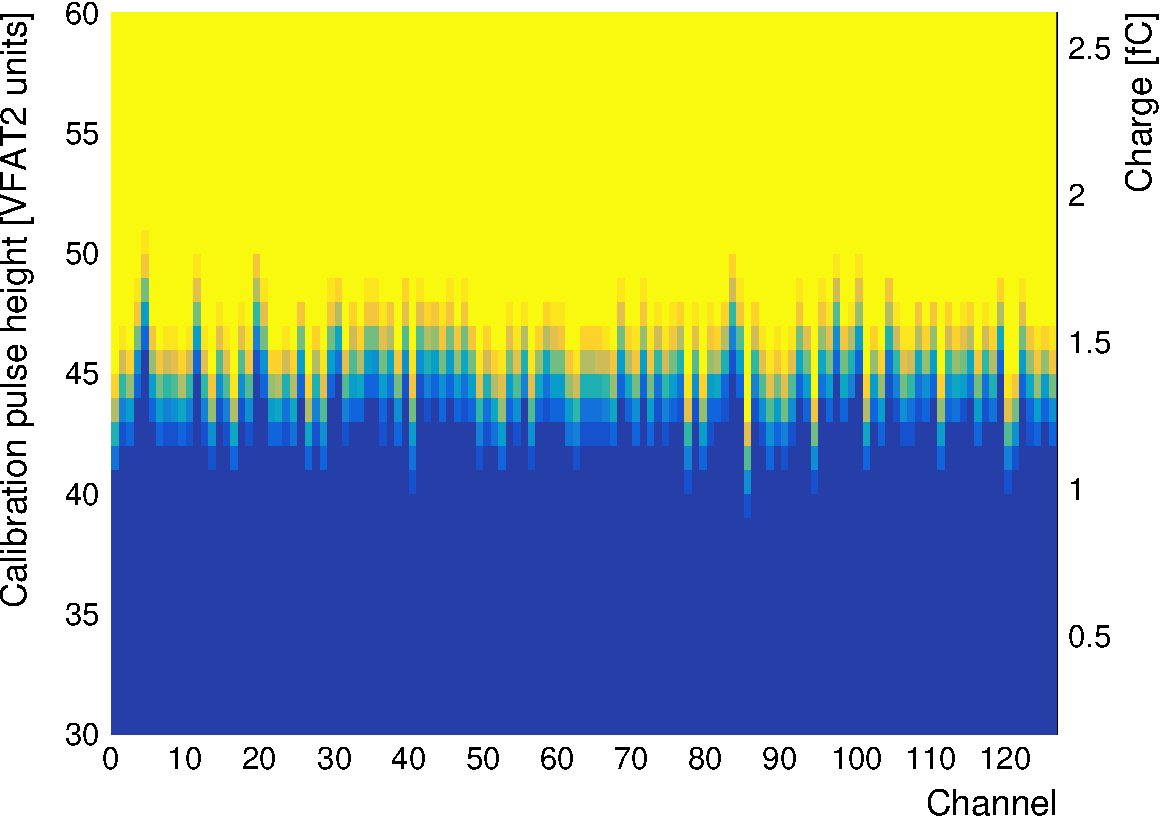
\includegraphics[width=0.49\textwidth]{img/plots/cSCurve_ChannelVCal_Trim0-crop}
        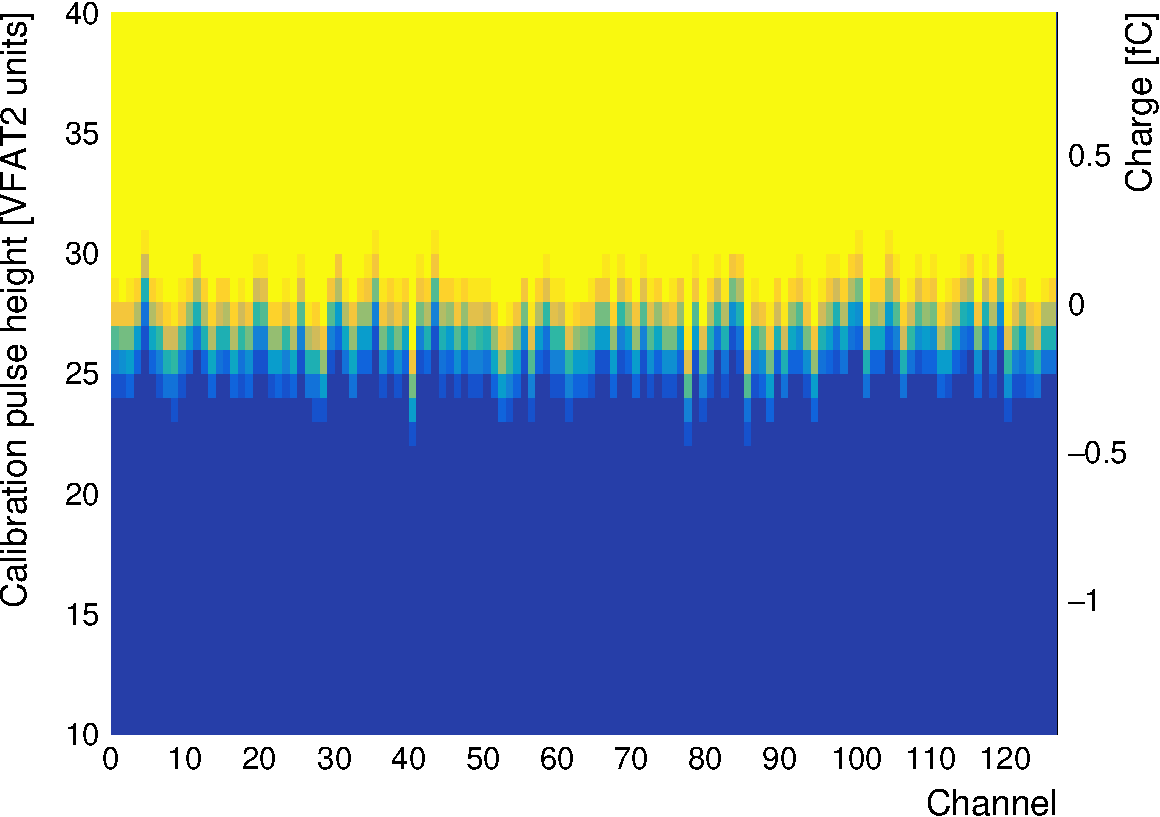
\includegraphics[width=0.49\textwidth]{img/plots/cSCurve_ChannelVCal_Trim1-crop}
        \caption{Plots of the s-curve scans for each channel with the minimum value of the channel registers on the left and the maximum value on the right.}
        \label{fig:II-4-trim}
      \end{figure}

      To align the channels, the average value of turn-on for both minimal and maximal value configuration is taken and set to be the aim of the equalization routine. For each channel, the script then sets its individual register value to the mean value and performs an s-curve scan. According to the turn-on value, the register is incremented or decremented and the procedure is repeated until the channel is aligned. The results of the alignment are shown in Figure \ref{fig:II-4-trimed} which plots the s-curve scan for each channel with the aligned values for the register on the left and the dispersion of the turn-on value for the non-aligned and aligned configurations. \\

      \begin{figure}[h!]
        \centering
        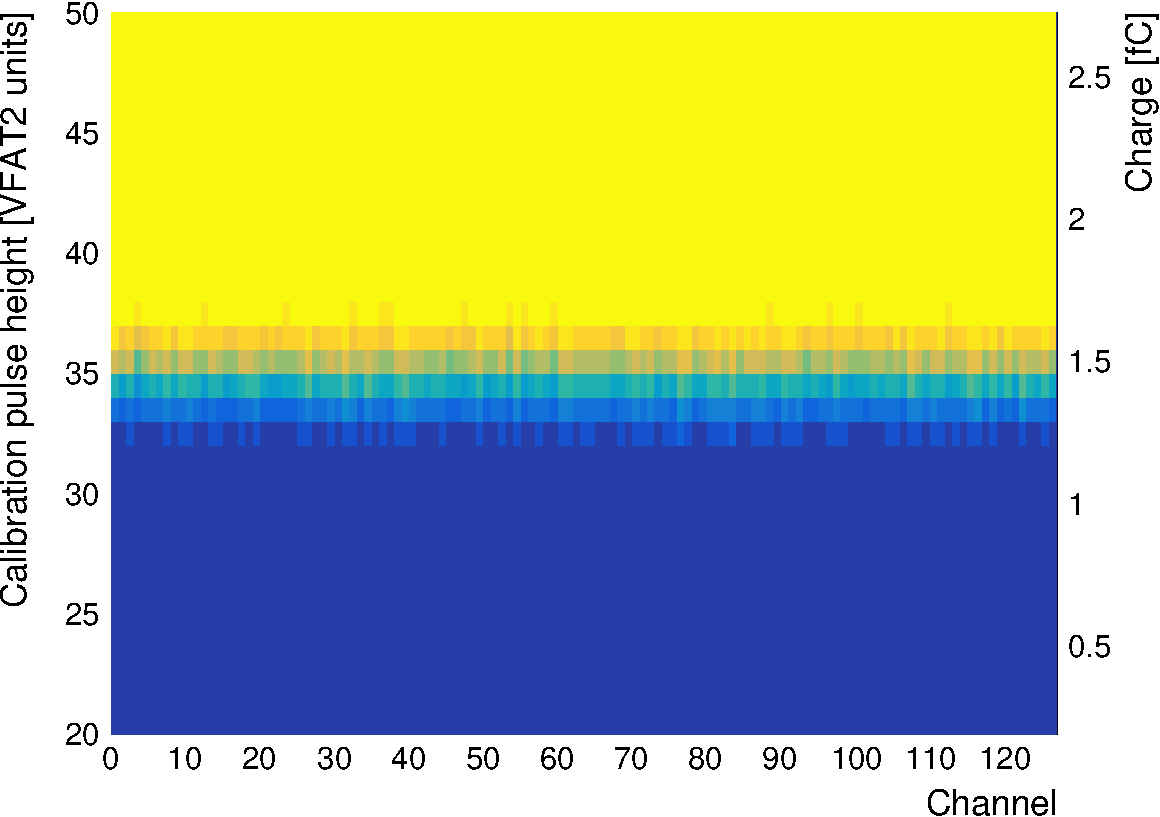
\includegraphics[width=0.49\textwidth]{img/plots/cSCurve_ChannelVCal_Trimed-crop}
        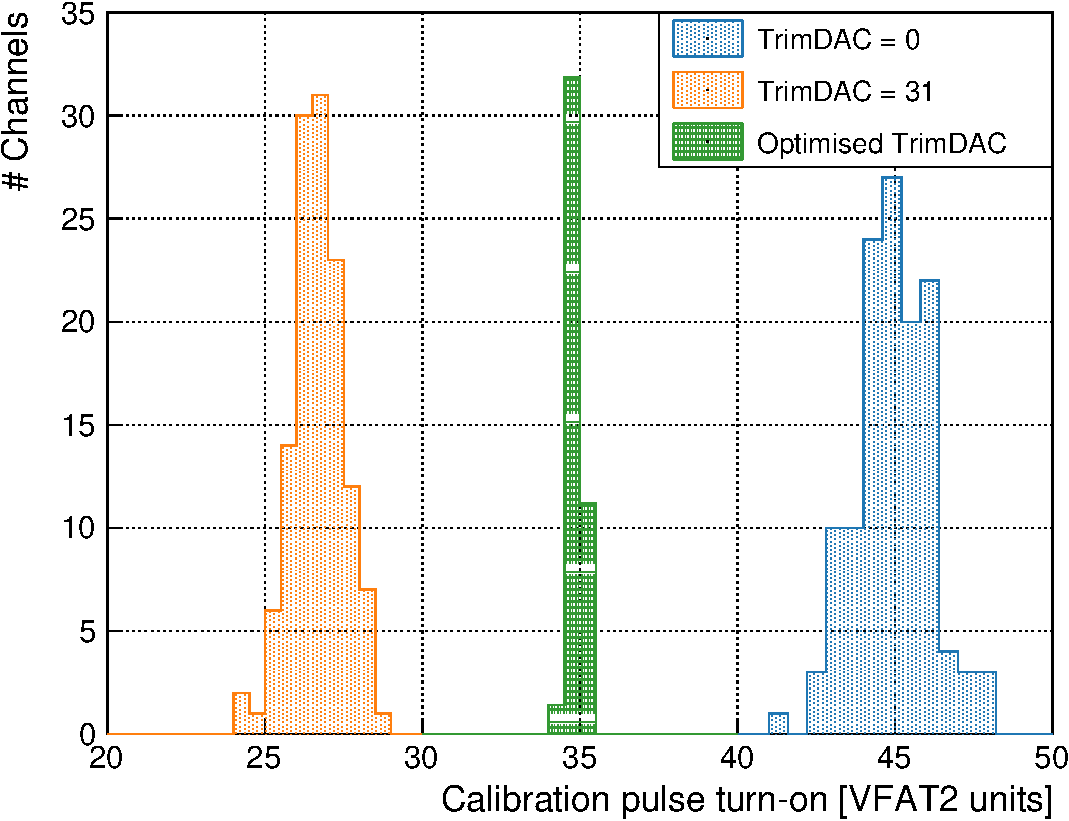
\includegraphics[width=0.49\textwidth]{img/plots/cSCurve_ChannelVCal_Disp-crop}
        \caption{Left: plot of the s-curve scan for each channel with the aligned values for the channel register. Right: dispersion of the turn-on value for the non-aligned (orange and blue) and aligned configurations (green, scaled by a factor of 0.35).}
        \label{fig:II-4-trimed}
      \end{figure}

      At the end of the script, the channels of the VFAT2 have all been tested against noise issues and have been adjusted so that they all display the same response to calibration pulses. The dispersion of the channels around the central value is improved from an initial value of 1.22 to a final value of 0.19 after alignment, corresponding to 0.10 fC and 0.02 fC respectively. This is the first time the full range of possibilities offered by the VFAT2 is used in a DAQ system and demonstrates that these features are within working specification.

    \section{Noise Measurement}

      A more quantitative comparison can be performed against \cite{Aspell:1069906} with respect to the electronic noise on the VFAT2. The latter will induce a smearing effect on the charge injected on the channel, either through noise on the voltage used to generate the pulse or on the electronics in the preamplification step. In a perfect system, the curve in Figure \ref{fig:II-4-scurve} would be a step function with values at 0 before the threshold is reached, and at 1 above. The noise is thus responsible for the steepness of the slope and defined as the sigma of the curve. After performing a fit of a logistic function, which is given in Equation \ref{eq:II-4-logistic}, the sigma is found to be 1.27 $\pm$ 0.02 VFAT2 Units. This value can be converted to femtocoulombs using the previous results and yields 0.10 $\pm$ 0.01 fC, which in turn can be expressed in terms of electrons to obtain
      \begin{equation}
        \sigma_e = 624 \pm 62 \ e^- \ .
      \end{equation}
      This can be compared to the value listed in the specification of the VFAT2 which is of 589 $\pm$ 84 $e^-$ when no detector is connected to the electronics. Both results are thus compatible within the error bars. \\

      The second measurement that can be performed is to study the variation of the noise from channel to channel. Figure \ref{fig:II-4-noise} plots the Equivalent Noise Charge (ENC), or noise in terms of electrons, for each channel. The distribution is centered around 622 $e^-$ with a spread of 31 $e^-$. Although the previously exposed procedure is able to align the mean of the s-curves, it does not affect their slope and thus noise. This parameter can not be changed and is intrinsic to the VFAT2.

      \begin{figure}[h!]
        \centering
        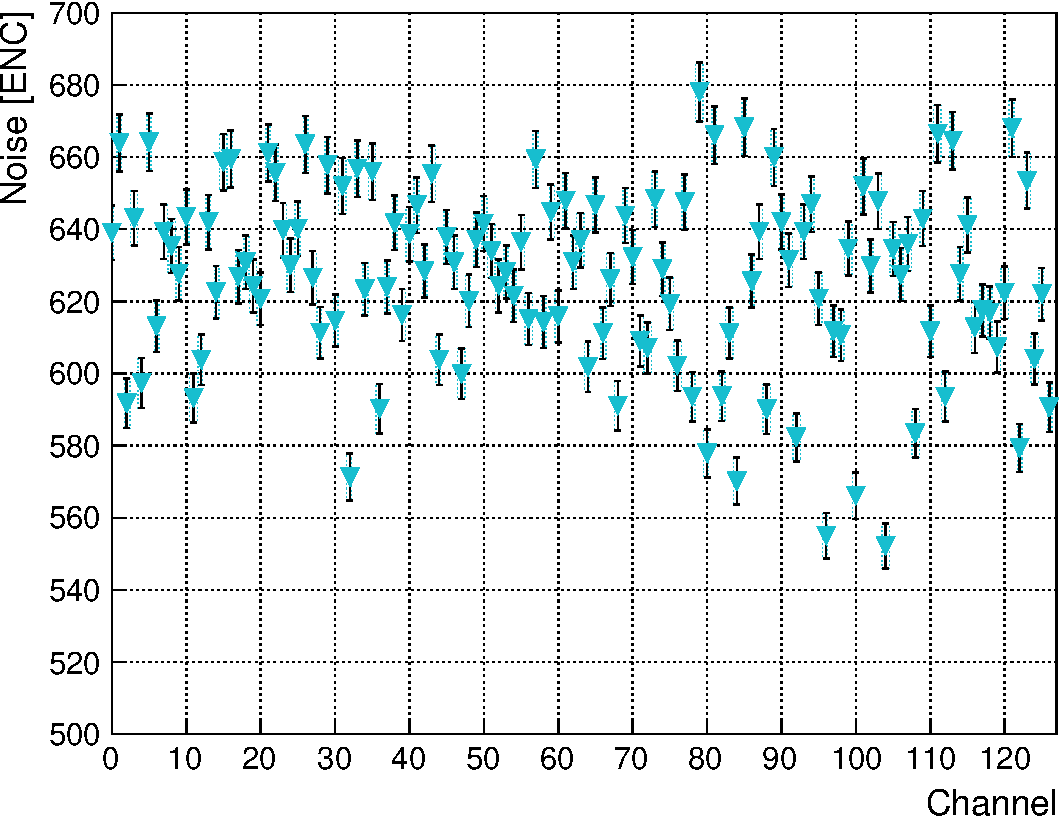
\includegraphics[width=0.49\textwidth]{img/plots/cEnoise_Disp-crop}
        \caption{Plots the equivalent noise charge for each channel.}
        \label{fig:II-4-noise}
      \end{figure}

  \section{Qualification of the GEB}

    In order to test the GEB, a small PCB equipped with the same connector as the VFAT2 Hybrids was developed. Using signals originating from the OptoHybrid, the board can check the integrity of the data and use on-board LEDs to indicate the results of the tests for the current position.

    \subsection{The GEB Testing Board}

      The PCB is a four layer board equipped with an FPGA and a microcontroller unit (MCU) to analyze the signals. Figure \ref{fig:II-4-geb-pcb} provides 3D models and a PCB layout of the board. Next to the processing units, the board also embarks an ADC, a DAC, a flash memory, a USB-to-SPI converter to link the universal serial bus (USB) port to the FPGA through serial peripheral interface bus (SPI), and powering options.

      \begin{figure}[h!]
        \centering
        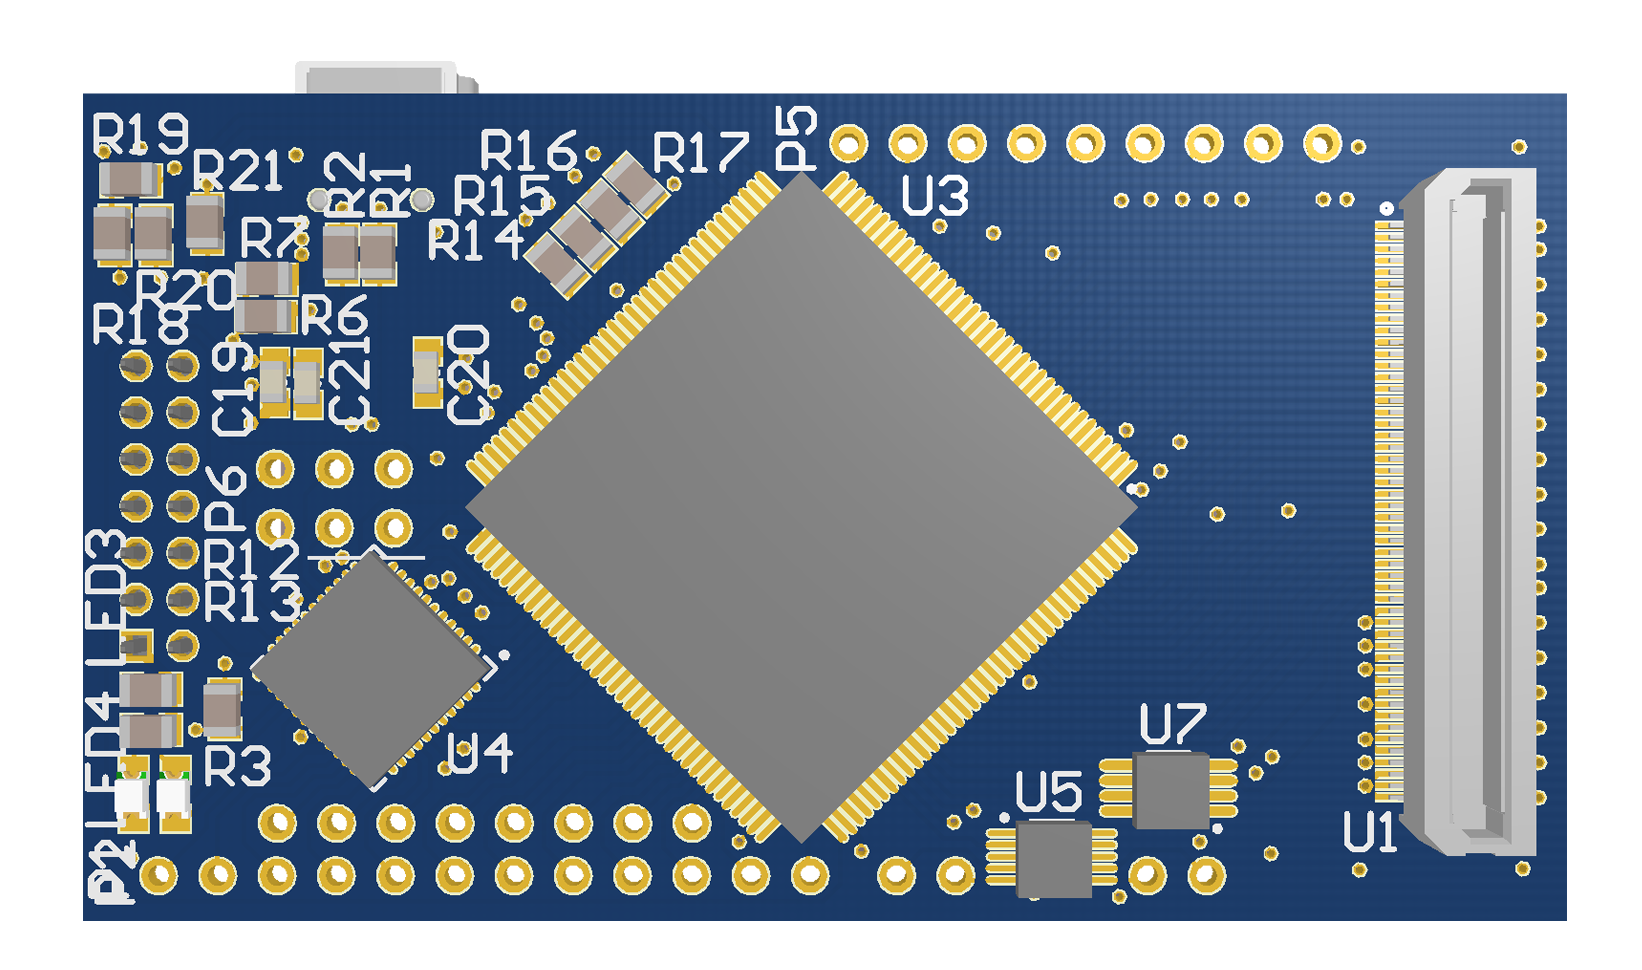
\includegraphics[width=0.49\textwidth]{img/II-4-qualification/geb-3d-0.png}
        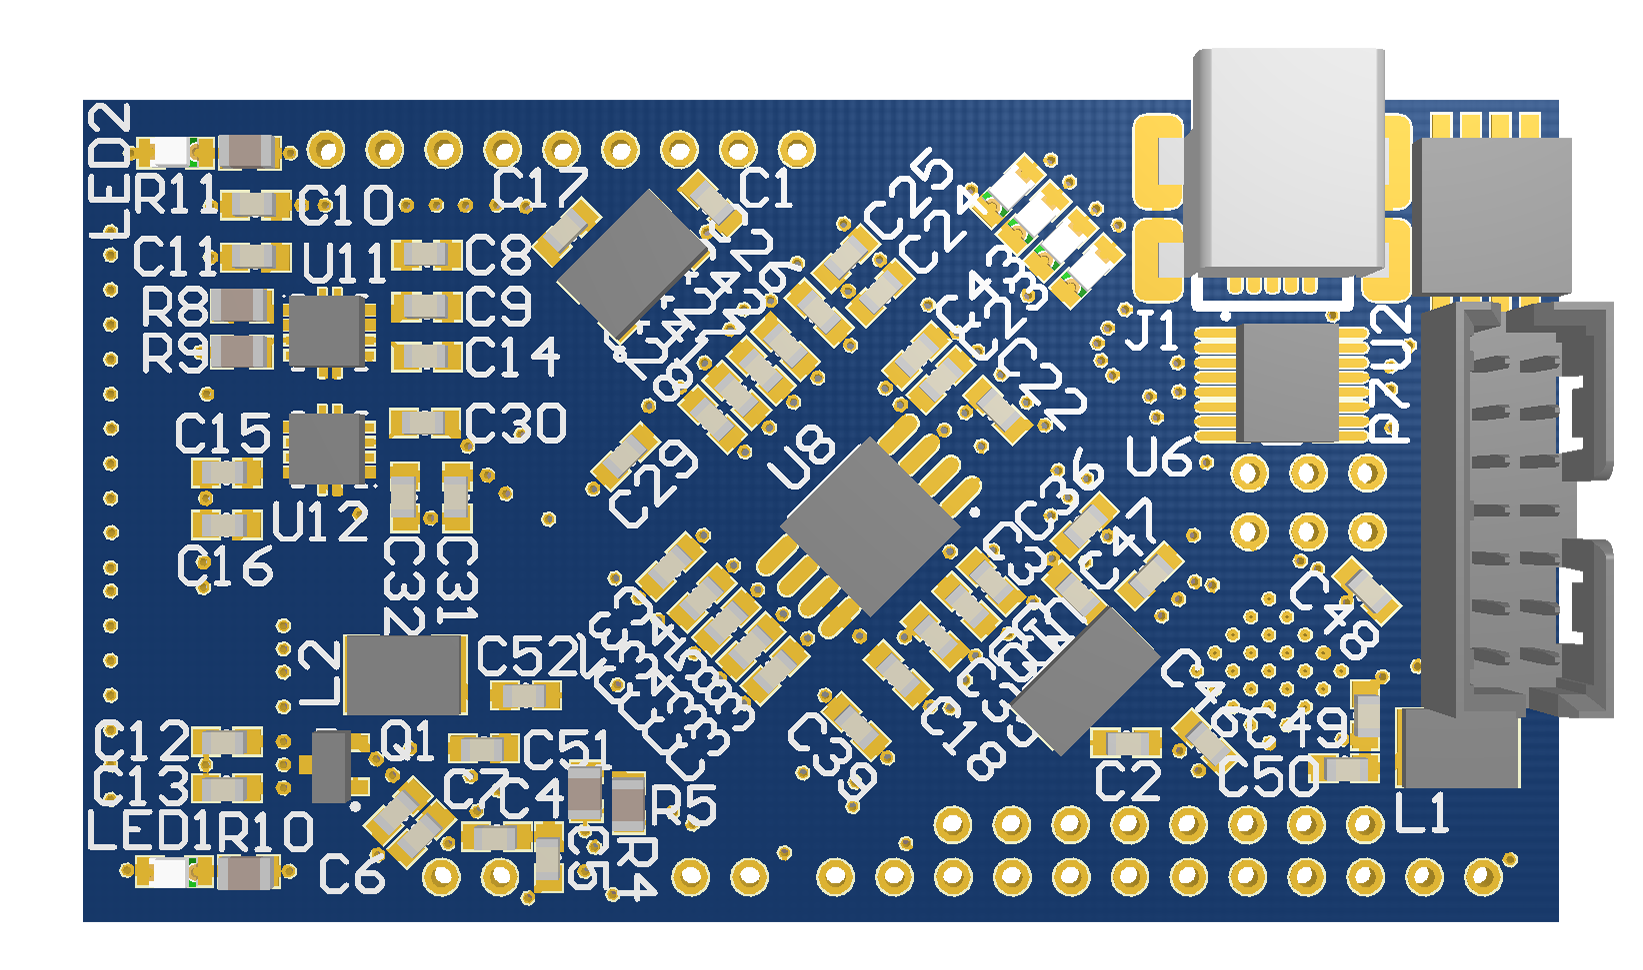
\includegraphics[width=0.49\textwidth]{img/II-4-qualification/geb-3d-1.png}
        \vspace*{0.3cm}
        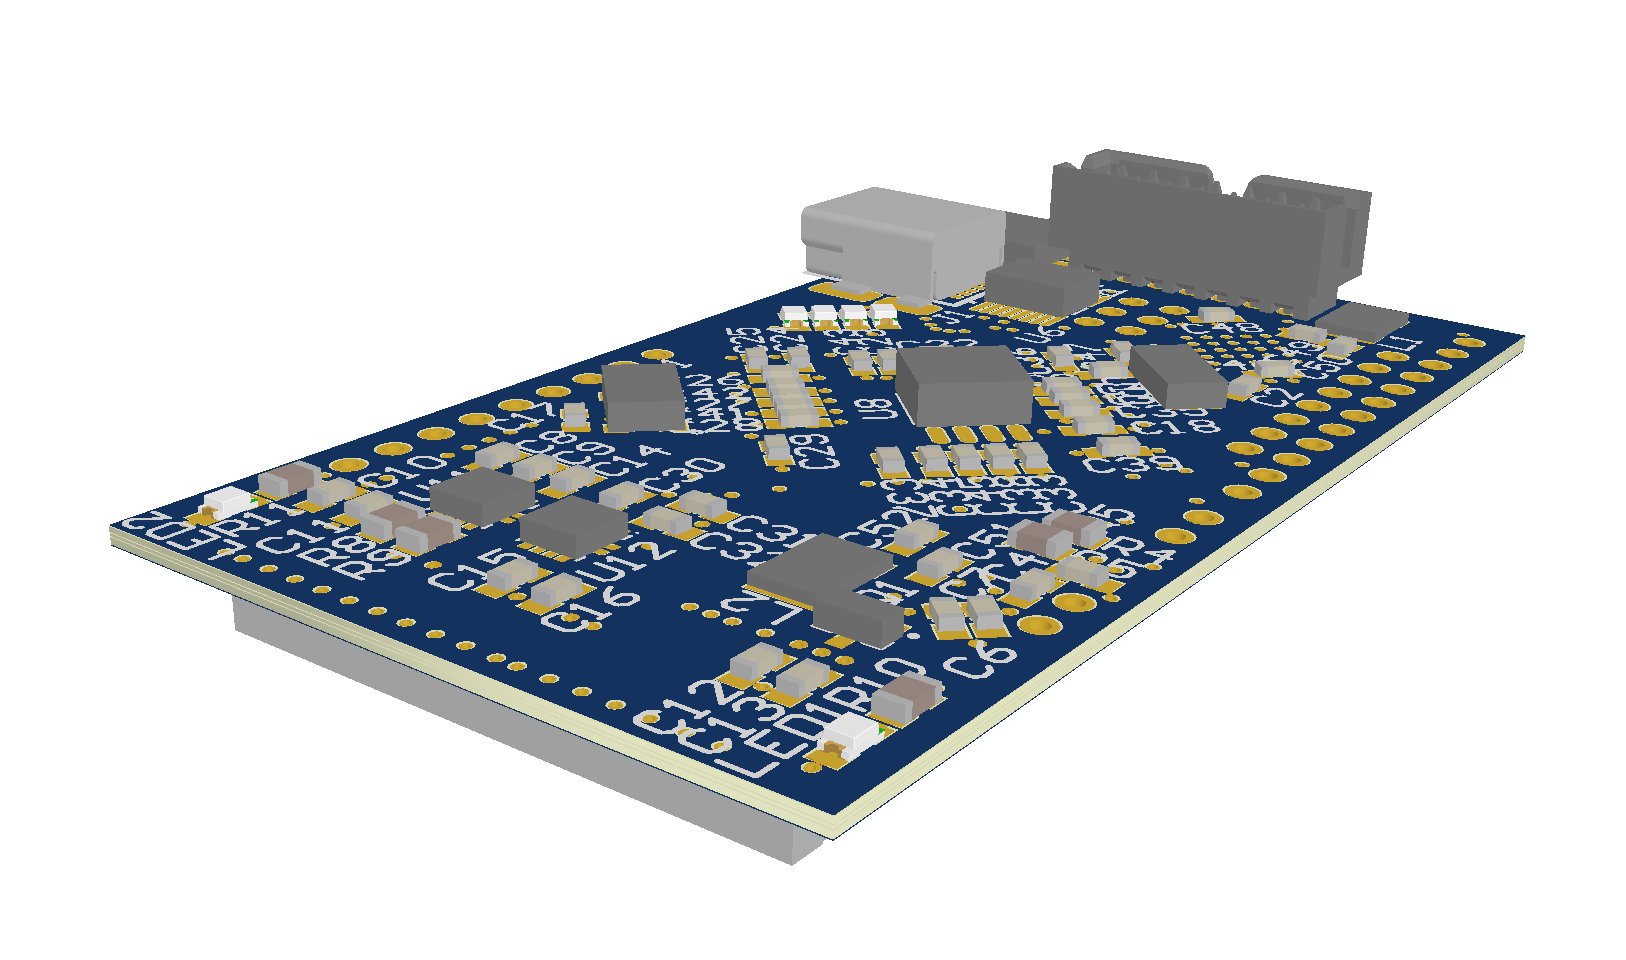
\includegraphics[width=0.49\textwidth]{img/II-4-qualification/geb-3d-2.png}
        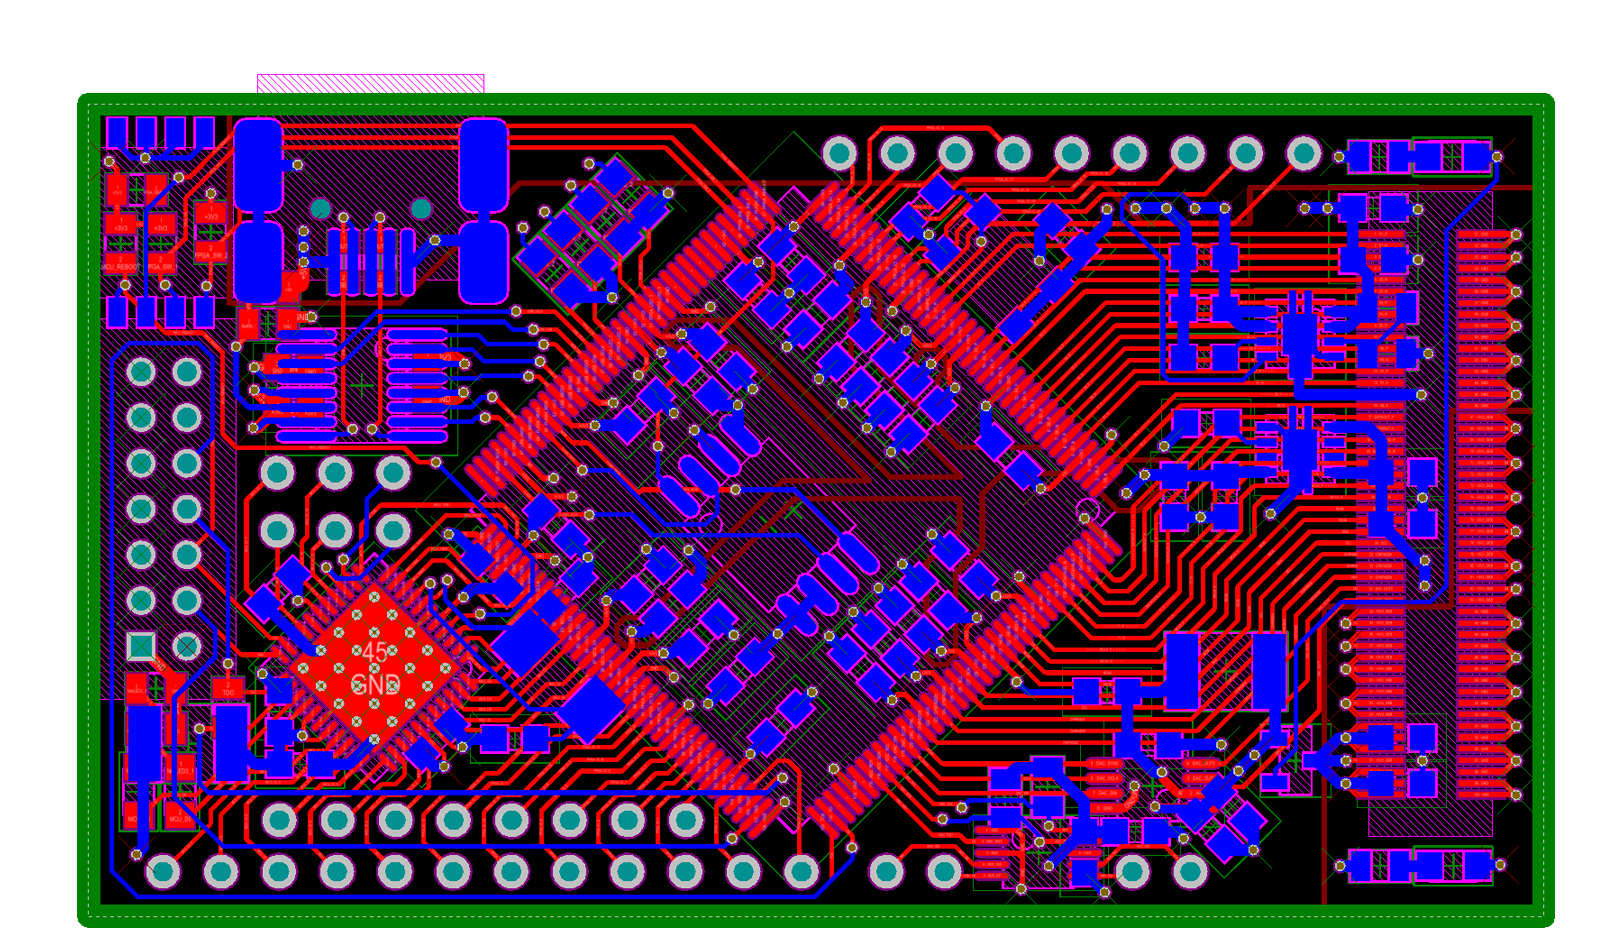
\includegraphics[width=0.49\textwidth]{img/II-4-qualification/geb-pcb.png}
        \caption{3D models and PCB layout of the GEB testing board.}
        \label{fig:II-4-geb-pcb}
      \end{figure}

      \paragraph{Powering of the board} is done either through the GEB connector which provides 2.5 V to the system or through the USB port. In case USB is used, the GEB power source is automatically disabled and 3.3 V is given to the system to increase processing speed. The 2.5 V or 3.3 V are further used to generate the 1.2 V required for the internal logic of the FPGA.

      \paragraph{The processing units} of the board, namely the Xilinx Spartan-6 FPGA (XC6SLX9-2TQG144C) and the ATMEL MCU (ATmega164PA), are what controls the various components. The FPGA is the main element of the board and is connected to all other chips. It can either control them directly or act as a router for the signals originating from the MCU. The communication between the two processing units is done via four serial buses: two universal asynchronous receiver/transmitter (UART), one SPI, and one bus composed of four GPIOs. Next to the links to the FPGA, the remaining 16 IOs of the MCU are broken out on header connectors for debugging purposes. The same is done for 22 IOs of the FPGA which are connected to headers.

      \paragraph{The GEB connector} holds 30 digital signals, 2 analog signals, and power and ground lines. The digital signals are all connected to the FPGA while the two analog signals are connected to the DAC.

      \paragraph{The USB port} is used to communicate with a computer using an FTDI chip (FT220XS) which converts the USB protocol to SPI.

      \paragraph{The analog part} of the board is controlled by the ADC (ADS1015) and the DAC (DAC8532). The two outputs of the DAC are connected to the GEB connector to drive the two analog signals digitized by the OptoHybrid. The ADC signals on the other hand are purely used for debugging purposes and connected to headers.

      \paragraph{Programming} the system is done through the Joint Test Action Group (JTAG) protocol which connects to the FPGA and the MCU. JTAG allows multiple devices to be connected in series and programs them both by shifting the configuration from one to another. The configuration scheme of the system can be modified to only affect the FPGA by removing a 0 $\Omega$ resistor which bypasses the MCU.

    \subsection{Testing the GEB}

      To test the GEB positions, the OptoHybrid is used to generate a pseudorandom binary sequence (PRBS) and transmit it over the data lines along with a reference clock. PRBS is often used to detect errors on communication lines including optical fibers. It relies on a sequence of bits to compute the next bit in the stream. A vector of bits is loaded in shift registers and is moved by one position every clock cycle. The overflowing position in transmitted on the line while the entering position is computed by summing the data stored in given positions. PRBS-7, for example, uses 7-bit-long vectors and computes the new element with
      \begin{equation}
        x_0 = x_6 \oplus x_5 \& x_1
      \end{equation}
      which yields a repetition period of pattern of 127 clock cycles. \\

      For each differential pair or single ended signal, a different seed is used for the PRBS-7 generator. By receiving the clock along with the data, the GEB tester board can decode the bit streams and ensure that the encoding is correct. In case one of the lines is faulty, the LEDs connected to the FPGA are used to display an error code. \\

      The analog lines are tested by generating a given voltage using the DAC. The OptoHybrid is then used to readout the value on the line and check the results are matching.

  \section{Qualification of the System}

    The final qualification procedure developed aims at testing the system in its entirety. Figure \ref{fig:II-4-script} provides a screen shot of the output of the script. The latter first attempts to establish communication with the GLIB/CTP7 and the OptoHybrid in section A and B. It then performs a series of read/write operations on the registers ensuring that every request receives a response in section C and D. Once the tests on the GLIB/CTP7 and OptoHybrid are done, the script detects all present VFAT2s in section E through I2C requests. Using these, random read/write operations are made on the registers of the VFAT2s in section F to test the reliability of the communication. Afterwards, in section G, chips are turned on one by one and tracking data is read out. The script verifies that the counters add up and that the data is not corrupted. Then, it performs the same action with all VFAT2s active at the same time in section H. The last test performed using the VFAT2s, in section I, is the maximum readout rate that can be achieved by the system. Finally, section J looks at the error rate on the optical links to ensure no errors appear on the communication lines. \\

    This test is used to test the system configuration and ensure that every component is configured correctly. It can detect errors at any level of the system, from the VFAT2s to the GLIB/CTP7.

    \begin{figure}[p!]
      { \footnotesize
\begin{alltt}
A. Testing the GLIB's presence
   Trying to read the GLIB board ID... If this test fails, the script
   will stop.
   > { \color{green} Passed... }

B. Testing the OH's presence
   Trying to set the OptoHybrid registers... If this test fails, the
   script will stop.
   > { \color{green} Passed... }

C. Testing the GLIB registers
   Performing single and FIFO reads on the GLIB counters and ensuring
   they increment.
   > { \color{green} Passed... }

D. Testing the OH registers
   Performing single and FIFO reads on the OptoHybrid counters and
   ensuring they increment.
   > { \color{green} Passed... }

E. Detecting the VFAT2s over I2C
   Detecting VFAT2s on the GEM by reading out their chip ID.
   Detected 18 VFAT2s: [1, ..., 23]

F. Testing the I2C communication with the VFAT2s
   Performing random read/write operation on each connect VFAT2.
   > { \color{green} Passed... #1 }
   { \color{gray} [...] }
   > { \color{green} Passed... #23 }

G. Reading out tracking data
   Sending triggers and testing if the Event Counter adds up.
   > { \color{green} Passed... #1 }
   { \color{gray} [...] }
   > { \color{green} Passed... #23 }

H. Reading out tracking data
   Turning on all VFAT2s and looking that all the Event Counters add up.
   > { \color{green} Passed... }

I. Testing the tracking data readout rate
   Sending triggers at a given rate and looking at the maximum readout
   rate that can be achieved.
   Maximum readout rate 200000 Hz

J. Testing the optical link error rate
   GLIB tracking link error rate is of          0 Hz
   GLIB trigger link error rate is of           0 Hz
   OptoHybrid tracking link error rate is of    0 Hz
   OptoHybrid trigger link error rate is of     0 Hz

K. Results
   A.    > { \color{green} Passed... }
   { \color{gray} [...] }
   J.    > { \color{green} Passed... }
\end{alltt} }
      \caption{Output of the qualification procedure developed to test the DAQ system in its entirety.}
      \label{fig:II-4-script}
    \end{figure}

  \section{Conclusion}

    For the first time, a method was developed to use the calibration capabilities of the VFAT2 to their full extend by taking advantage of the channel by channel optimization. The procedure we designed to qualify the VFAT2s is used to detect faulty units and perform qualification tests which entirely characterize the analog front-end of each VFAT2. The first part of the results can be compared to the specifications of the VFAT2 and yields the range of charge that can be injected on the channels and the noise on the VFAT2. The former results in a range of -0.9 fC to 20 fC while the latter was found to be of 624 $\pm$ 62 e$^-$. This is in turn used to provide information on the effective threshold applied on the channels in terms of electrons and thus induced charge. The second part of the script aligns the response of each channel around a central value and reduces the threshold disparity from an initial dispersion value of 1.22 to a value 0.19 after alignment in VFAT2 units, corresponding to 0.10 fC and 0.02 fC respectively. \\

    Qualification procedures were also created for the GEB, for which we designed a GEB testing board to test each position and detect broken lines. The board relies on an FPGA coupled with an MCU to communicate with the OptoHybrid and test the integrity of the transmitted signals. The results of each test are displayed using on-board LEDs and inform the user of the quality of the signals and thus the GEB. \\

    Finally, we tested the system as a whole using a script which targets specific components of the architectures. Random read/write operations to the GLIB/CTP7, OptoHybrid, and VFAT2s are performed, tracking data is read out, and stress tests are done to push the system to the limit. A report is provided to the user about each individual point in order to qualify the system or not. \\

    These tools are used for the preparation of the slice test to select appropriate components and install testing facilities at CERN and in other associated research laboratories.
